\section{Monetary Models - Background}

\begin{frame}

\begin{center}
{\LARGE Monetary Models - Background}
\end{center}

\end{frame}

%-------------------------------------------------------
\subsection{History Lesson}
%-------------------------------------------------------

\begin{frame}{Quantity theory of money}

Much discussion (though not in recent years) of the effects of monetary policy began with some form of the following equation
\begin{equation}
M_{t}V_{t} \equiv P_{t}Y_{t} \label{eqn:mvpy}
\end{equation}
where $M_{t}$ is the quantity of money, $V_{t}$ the velocity of its circulation, $P_{t}$ the general price level and $Y_{t}$ real output.

\vspace{2mm}
Equation (\ref{eqn:mvpy}) is an \emph{identity} (always true by definition)
\begin{itemize}
\item Holds regardless of CB targeting interest rate, $i_{t}$, or $M$ directly
\item Uninteresting unless a theory restricts behavior of at least one variable
\end{itemize}

\vspace{2mm}
(Long run) `classical dichotomy' / `quantity theory of money'
\begin{itemize}
\item In the long run, $Y$ and $V$ are determined by non-monetary factors
\item Thus, M and P move 1:1 in the long run
\end{itemize}

\end{frame}

%-------------------------------------------------------

%-------------------------------------------------------

\begin{frame}{Quantity theory of money}

Economists agree about little but\ldots
\begin{itemize}
\item 	The \emph{long run} classical dichotomy is arguably an exception
\item 	Long run growth determined by `supply' factors - not monetary
\item 	In LR, monetary factors only influence \emph{nominal}, but not \emph{real} variables
\item	Long run correlations between $M$ and $P$ $\approx 1$ in the data
\end{itemize}

\vspace{2mm}
Almost complete consensus that \emph{`there is no long-run trade-off between the rate of inflation and the rate of unemployment'} - Taylor (1996)
%\begin{itemize}
%\item	Caveat: Zero lower bound and the probability of monetary policy being constrained in low inflation environments
%\item	Caveat: High inflation may correlate with volatile inflation and mismanaged policy affecting economic activity
%\item	But the long run classical dichotomy is generally thought of as a given
%\end{itemize}

\end{frame}

%-------------------------------------------------------

%-------------------------------------------------------

\begin{frame}{Fisher equation}

Its rare nowadays for central banks to use $M_{t}$ as an explicit policy tool
\begin{itemize}
\item	Typically now set a short term nominal interest rate, $i_{t}$
\item	Given `money demand', the central bank adapts money supply so market clears at desired $i_{t}$
\end{itemize}

\vspace{2mm}
In this context, the `quantity equation' is less intuitive - instead the `Fisher equation' is useful to aid understanding
\begin{eqnarray}
i_{t} = r_{t} + E_{t}[ \pi_{t+1} ] 
\end{eqnarray}
where $i_{t}/r_{t}$ is the nominal/real interest rate and $\pi_{t}$ is (net) inflation.

\vspace{2mm}
The (long run) classical dichotomy implies that $r_{t}$ is unrelated to monetary factors
\begin{itemize}
\item	$i_{t}$ and inflation move 1:1, conditional on $r_{t}$
\item	If $r_{t}$ changes without a change in $i_{t}$ inflation adjusts
\end{itemize}

\end{frame}

%-------------------------------------------------------
\subsection{Effects of Monetary Policy}
%-------------------------------------------------------

\begin{frame}{Interaction of real and nominal factors}

In the shorter run the classical dichotomy is not broadly accepted
\begin{itemize}
\item 	Money/interest rates and output (or other measures of activity, such as unemployment) appear to co-move
\item	Central banks' activities are predicated on the assumption that changing $i_{t}$ induces a change in $r_{t}$
\end{itemize}

\vspace{2mm}
Co-movements are suggestive that there is a connection between real and nominal variables (see Ch. 1 Walsh)
\begin{itemize}
\item	Lead-lag correlations $\Rightarrow$ high $M_{t}$ typically precedes high $Y_{t}$
\item	Cyclical movements in money track those of GDP growth fairly well until early 80s
\item	Short term nominal rates generally track - and somewhat precede - cyclical movements in GDP
\end{itemize}
 
\end{frame}

%-------------------------------------------------------

%-------------------------------------------------------

\begin{frame}{Interaction of real and nominal factors}

\begin{figure}[!htb]
\center{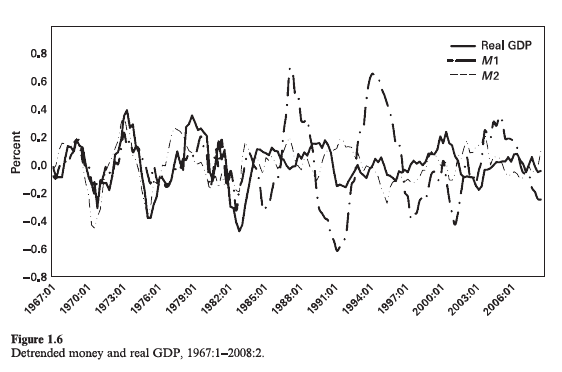
\includegraphics[width=0.8\textwidth]{Figures/detrend_M_and_GDP_walsh_ch1.png}}
\caption{\label{fig:walsh_ch1_M_GDP} De-trended money and output (from Walsh Ch.1)}
\end{figure}
 
\end{frame}

%-------------------------------------------------------

%-------------------------------------------------------

\begin{frame}{Interaction of real and nominal factors}

\begin{figure}[!htb]
\center{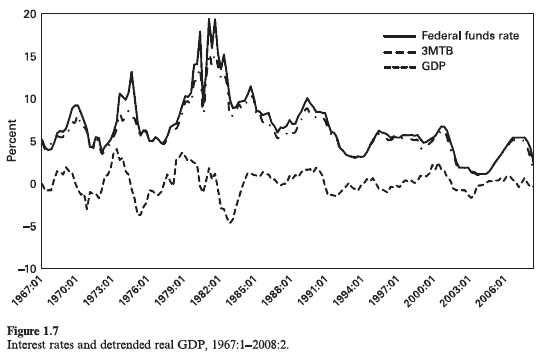
\includegraphics[width=0.8\textwidth]{Figures/i_rate_detrend_gdp_walsh_ch1.png}}
\caption{\label{fig:walsh_ch2_M_GDP} Short rate and de-trended output (from Walsh Ch.1)}
\end{figure}
 
\end{frame}

%-------------------------------------------------------

%-------------------------------------------------------

\begin{frame}{Interaction of real and nominal factors}

Difficult to disentangle direction of causality
\begin{itemize}
\item	Are these movements \emph{induced} by monetary policy or is policy \emph{responding} to the economy?
\item	Even if policy variable appears to lead activity, we face the \emph{post hoc ergo propter hoc} fallacy
\end{itemize}

\vspace{2mm}
Want to examine periods after an unanticipated `shock' from policymakers
\begin{itemize}
\item	Derives purely from policymaker - not economy - and thus closer to a `natural experiment'
\item	Then estimate propagation of shock through economy
	\begin{itemize}
	\item	If $M_{t}$ is the tool, does it affect $M/P$ and real activity, rather than passing 1:1 into prices? - Recall `quantity theory'
	\item	If $i_{t}$ is the tool, does it affect $r_{t}$ and real activity, rather than passing 1:1 into $E_{t}[\pi_{t+1}]$? - Recall Fisher equation
	\end{itemize}
%\item	May be possible to combine with a model to estimate `structural parameters' (more on this later\ldots)
\end{itemize}

\end{frame}

%-------------------------------------------------------

%-------------------------------------------------------

\begin{frame}{Identifying monetary policy shocks and their effects}

Friedman and Schwarz (1963) and narrative approaches
\begin{itemize}
\item Seminal work on influence of monetary policy in the U.S. (most notably in the Great Depression)
	\begin{itemize}
	\item	Documentary evidence to isolate $\Delta M$ unrelated to economic conditions
	\item	Suggests that fluctuations in money supply led to those in real activity
	\item	Related to case study analyses of disinflationary policy (Sargent (1986))
	\end{itemize}
\item Influential - but problematic elements in empirical approach
	\begin{itemize}
	\item 	Later support from Romer and Romer (1989) in a more modern form
	\item	Further strengthened by Romer and Romer (2004)
	\end{itemize}
\end{itemize}

\vspace{2mm}
Other recent work on obtaining measures of policy surprises
\begin{itemize}
\item	Nakamura and Steinsson (2013) and Gertler Karadi (2015) use `high frequency information'
\item	Look at asset price movements in short intervals around FOMC announcements to identify `surprises'
\end{itemize}

\end{frame}

%-------------------------------------------------------

%-------------------------------------------------------

\begin{frame}{Identifying monetary policy shocks and their effects}

\begin{quotation}
On three occasions the System deliberately took policy steps of major magnitude which cannot be regarded as necessary or inevitable economic consequences of contemporary changes in money income and prices. Like the crucial experiments of the physical scientist, the results are so consistent and sharp as to leave little doubt about their interpretation. The dates are January-June 1920, October 1931, and June 1936-January 1937
\end{quotation}
\center - Friedman and Schwarz, 1963, p.688

\end{frame}

%-------------------------------------------------------

%-------------------------------------------------------

\begin{frame}{Identifying monetary policy shocks and their effects}

\begin{quotation}
There was another major anti-inflationary shock to monetary policy on October 6, 1979. In effect, the Federal Reserve decided that its measures over the previous year had been unsuccessful in reducing inflation and that much stronger measures were needed. Although the shift in policy was to some extent presented as a technical change, the fact that it was intended to lead to considerably higher interest rates and lower money growth was clear. For example, "the Committee anticipated that the shift . . . would result in ... a prompt increase ... in the federal funds rate"
\end{quotation}
\center - Romer and Romer, 1989, p.142

\end{frame}

%-------------------------------------------------------

%-------------------------------------------------------

\begin{frame}{Identifying monetary policy shocks and their effects}

Friedman and Schwarz (1963) and narrative approaches
\begin{itemize}
\item Seminal work on influence of monetary policy in the U.S. (most notably in the Great Depression)
	\begin{itemize}
	\item	Documentary evidence to isolate $\Delta M$ unrelated to economic conditions
	\item	Suggests that fluctuations in money supply led to those in real activity
	\item	Related to case study analyses of disinflationary policy (Sargent (1986))
	\end{itemize}
\item Influential - but problematic elements in empirical approach
	\begin{itemize}
	\item 	Later support from Romer and Romer (1989) in a more modern form
	\item	Further strengthened by Romer and Romer (2004)
	\end{itemize}
\end{itemize}

\vspace{2mm}
Other recent work on obtaining measures of policy surprises
\begin{itemize}
\item	Nakamura and Steinsson (2013) and Gertler Karadi (2015) use `high frequency information'
\item	Look at asset price movements in short intervals around FOMC announcements to identify `surprises'
\end{itemize}

\end{frame}

%-------------------------------------------------------

%-------------------------------------------------------

\begin{frame}{Vector Autoregressions}

Another powerful approach to assessing the impact of monetary policy shocks is Vector Autoregression (VAR) analysis (see Walsh Ch. 1 for this example)

\vspace{3mm}
\begin{quotation}
While researchers have disagreed on the best means of identifying policy shocks, there has been a surprising consensus on the general nature of the economic responses to monetary policy shocks. A variety of VARs estimated for a number of countries all indicate that, in response to a policy shocks, output follows a hump-shaped pattern in which the peak impact occurs several quarters after the initial shock.
\end{quotation}
\begin{center}
- Walsh, 1998, p.31
\end{center}

\vspace{3mm}
See discussion in lecture 1

\end{frame}

%-------------------------------------------------------

%-------------------------------------------------------

\begin{frame}{Vector Autoregressions}

\begin{figure}[!htb]
\center{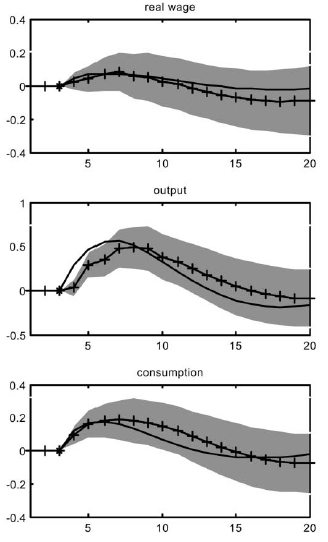
\includegraphics[width=0.30\textwidth]{Figures/cee2005_fig1_subset2}}
\caption{\label{fig:cee05_2} Subset of IRFs from CEE (2005)}
\end{figure}

\end{frame}

%-------------------------------------------------------

%-------------------------------------------------------

\begin{frame}{Vector Autoregressions}

\begin{figure}[!htb]
\center{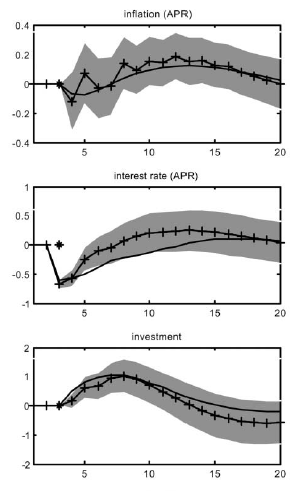
\includegraphics[width=0.30\textwidth]{Figures/cee2005_fig1_subset1}}
\caption{\label{fig:cee05_1} Subset of IRFs from CEE (2005)}
\end{figure}

\end{frame}

%-------------------------------------------------------

%-------------------------------------------------------

\begin{frame}{Vector Autoregressions}

VAR approach useful but not without flaws/critics\ldots
\vspace{2mm}
\begin{itemize}
\item 	Monetary policy shocks are now likely rare/small (Ramey (2016))
	\begin{itemize}
	\item	Makes it more difficult to use \emph{policy} shocks to estimate impact of policy
	\item	Can still estimate role of policy but need \emph{other} shocks \textbf{and} a model
	\end{itemize}
\vspace{1mm}
\item	Changes in underlying parameters (Lucas critique and Rational Expectations)
	\begin{itemize}
	\item	Response to shocks depends on parameters describing policymakers' approach \textbf{and} all other parameters in the economy (e.g. regulation, preferences\ldots)
	\item	If they change, previous estimates may become obsolete
	\end{itemize}
\vspace{1mm}	
\item 	Responses may not be accurately recovered even from data generated by a model (Chari \emph{et al} (2008))
	\begin{itemize}
	\item	Can still use, but in a `moment matching' exercise \emph{involving a model}
	\item	VARs on actual data and on data from model - minimize discrepancy
	\end{itemize}
\end{itemize}

\end{frame}

%-------------------------------------------------------

%-------------------------------------------------------

\begin{frame}{Vector Autoregressions}

More problems with VAR analysis\ldots
\vspace{2mm}
\begin{itemize}
\item	Unhelpful for welfare analysis
	\begin{itemize}
	\item	Knowing that policy affects activity is one thing\ldots
	\item 	\ldots but knowing \emph{how it should try to affect it} is another
	\item 	Agent's optimization problems must be explicit for micro-founded welfare analysis
	\item 	VARs are silent on this
	\end{itemize}
\item	Story telling / incorporation of microeconomic evidence
	\begin{itemize}
	\item 	Policymakers like to understand/explain transmission mechanism
	\item	Elements of models (such as, say, household risk aversion) can be pinned down by evidence from experiments/more granular research
	\item	Not possible with VARs (or very difficult)
	\end{itemize}
\end{itemize}

\vspace{2mm}
A lot of these `problems' can be addressed by using a model\ldots

\end{frame}

%-------------------------------------------------------
\subsection{DSGE Models}
%-------------------------------------------------------

\begin{frame}{Role of monetary policy - DSGE models}

DSGE models initially associated with the `Real Business Cycle' literature
\begin{itemize}
\item	Seminal work of Kydland and Prescott (1982) and Prescott (1986)
\item	No (or minor) distortions $\Rightarrow$ despite fluctuations (the `business cycle') the economy is always efficient
\item	Limited role of monetary policy - main shocks were `real' (technology)
\end{itemize}

\vspace{2mm}
Beautiful models - but unsatisfactory in various dimensions
\begin{itemize}
\item	If monetary policy was included, optimal policy looked nothing like real world practice
\item	Effects of policy shocks often counterfactual (recall evidence discussed above)
\item	Hard to reconcile dominant role of technology shocks with\ldots
	\begin{itemize}
	\item	\emph{Unconditional} positive comovement of employment and output in data
	\item	Empirical studies $\Rightarrow$ \emph{technology} shocks move them in opposite direction
	\end{itemize}
\end{itemize}

\end{frame}

%-------------------------------------------------------

%-------------------------------------------------------

\begin{frame}{Role of monetary policy - DSGE models}

The challenge:
\begin{itemize}
\item	Keep the `good' aspects of RBC models\ldots
\item	\ldots while enhancing ability to explain and justify monetary policy
\end{itemize}

\end{frame}

%-------------------------------------------------------

%-------------------------------------------------------

\begin{frame}{Role of monetary policy - DSGE models}

New Keynesian modeling was a response to this challenge
\vspace{2mm}
\begin{itemize}
\item	Interpret as a \textbf{micro-founded} formalization of `Keynesian' ideas
	\begin{itemize}
	\item	IS-LM analysis `much less careful' - rather \emph{ad hoc}
	\item	`We are an equation short' (Keynes) - price setting not modeled
	\end{itemize}
\vspace{1mm}
\item	Emphasis on \textbf{nominal rigidities} as a reason for fluctuations
	\begin{itemize}
	\item	Empirical evidence of significant price (incl. wage) stickiness
	\item	Taylor (1999), Bewley (1999), Dhyne \emph{et al} (2006), Nakamura and Steinsson (2008)\ldots
	\end{itemize}
\vspace{1mm}	
\item	(Very) loosely - sticky prices $\Rightarrow$ \textbf{Classical Dichotomy broken}
	\begin{itemize}
	\item	$\Delta M_{t}$ shock doesn't \emph{immediately} pass 1:1 to prices
	\item	$\Delta i_{t}$ shock doesn't \emph{immediately} pass 1:1 to $E_{t}[\pi_{t+1}]$ - thus $r_{t}$ changes
	\end{itemize}
\vspace{1mm}	
\item	Explicit distortions from \textbf{imperfect competition} and sticky prices implies \textbf{economy not fully efficient}
	\begin{itemize}
	\item	Scope for policy to be welfare-enhancing
	\end{itemize}
\end{itemize}

\end{frame}

\end{document}
